\documentclass{article}
\usepackage{graphicx} % Required for inserting images
\usepackage{subcaption}
\usepackage{amsmath, amssymb, booktabs}
\usepackage{hyperref}
\usepackage{comment}
\graphicspath{ {./figures/} }
\usepackage{xcolor}  % Required for color customization
\hypersetup{
  colorlinks=true,  % Activates colored links
  linkcolor=blue,   % Color of internal links (sections, pages, etc.)
  citecolor=blue,   % Color of citation links
  urlcolor=blue     % Color of external links (URLs)
}

\title {}
% \title{Raisin the Bar from Linear Regression to Generalized Linear Models}
\author{Johnathan Ferdinand, Devina Gera, Archimedes Li, Henry Liu, \\Katherine Shi, Sam Stevens}
\date{\today}
\begin{document}
\maketitle

\section{Analysis}
We can see that the price increases over time despite showing volitility. The mean and variance change over time so the stock price is not stationary. (Figure \ref{fig:stockPrices}).

\noindent We then ran the Augmented Dickey-Fuller test on the data and got the following output:
\begin{verbatim}
Dickey-Fuller = -3.1858, Lag order = 19, p-value = 0.09026
alternative hypothesis: stationary
\end{verbatim}
We get a P value of $0.09$, thus we fail to reject the null hypothesis, and the Price of the stock is non-stationary.


\noindent Figure \ref{fig:return} gives that the average return on CAT is $0$. At a quick glance, we can see that the mean is approximately 0 (fig \ref{fig:return}\subref{fig:returnCat}). The histogram showing a normal distribution with mean 0 confirms our suspicions (fig \ref{fig:return}\subref{fig:returnHisto}).

\noindent We ran the same test again for the return of the stock and got the following output:
\begin{verbatim}
Dickey-Fuller = -20.102, Lag order = 19, p-value = 0.01
alternative hypothesis: stationary
\end{verbatim}
This time, we reject the null hypothesis, so the return on the stocks is non-stationary.

\noindent The ACF shows that the return series is not dependent on the previous day's error.
          The PACF shows that the return series autocorrelates with lags.
	  Thus, the Return series are influenced by previous days Return.(Figure \ref{fig:acf})

	  \noindent The absence of autocorrelation is confirmed by the Box-Ljung test, which gives an output of 
	  \begin{verbatim}
	  X-squared = 7.3365, df = 1, p-value = 0.006757
	  \end{verbatim}
We reject the null hypothesis,  thus the return series is not independent.

\noindent The plot of ACF of square return values (Fig \ref{fig:acfErr}) shows a clear but slow decay of auto correlation.

\noindent The rolling performance chart points to GARMA being able to improve our ARMA model. (Fig \ref{fig:volatility})

\begin{figure}
	\centering
	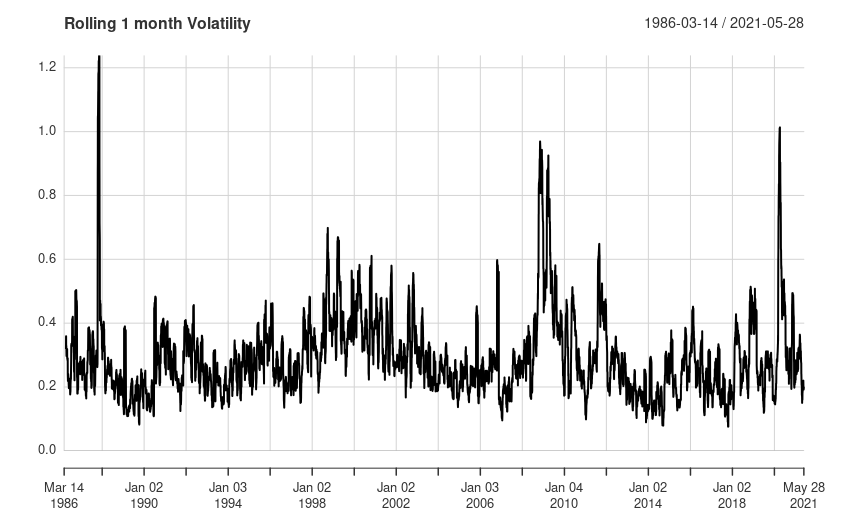
\includegraphics[width=\linewidth]{monthly_volatility}
	\caption{Rolling 1 month volatility for CAT.}
	\label{fig:volatility}
\end{figure}
\begin{figure}
	\centering
	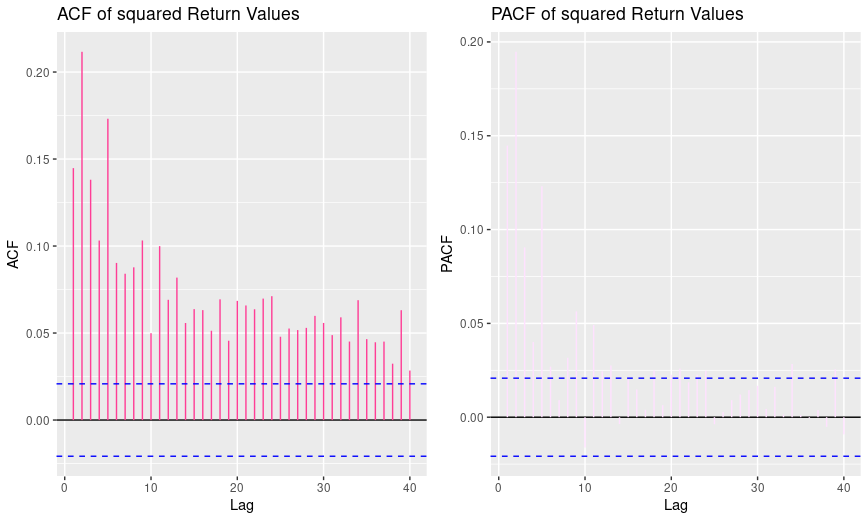
\includegraphics[width=\linewidth]{acf_pacf_squared}
	\caption{ACF of return values (left) and PACF of return values(right)}
	\label{fig:acfErr}
\end{figure}

\begin{figure}
	\centering
	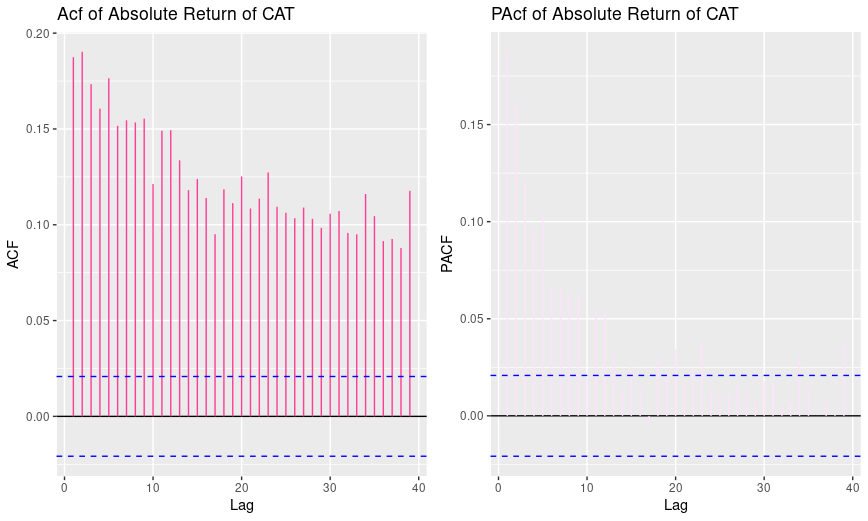
\includegraphics[width=\linewidth]{acf_pacf_of_cat}
	\caption{ACF of return values (left) and PACF of return values(right)}
	\label{fig:acf}
\end{figure}

\begin{figure}
	\centering
	\begin{subfigure}{\linewidth}
		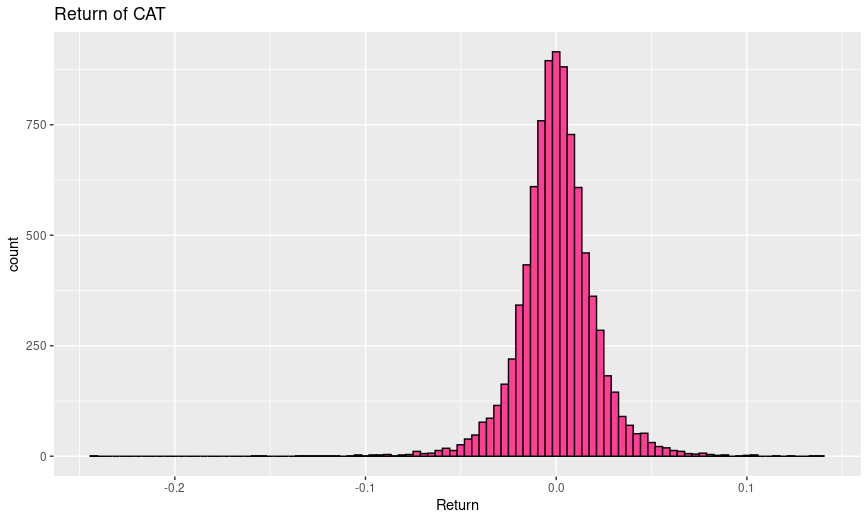
\includegraphics[width=\linewidth]{return_of_cat_histo}
		\caption{Histogram for fig \ref{fig:returnCat}}
		\label{fig:returnHisto}
	\end{subfigure}
	\centering
	\begin{subfigure}{\linewidth}
		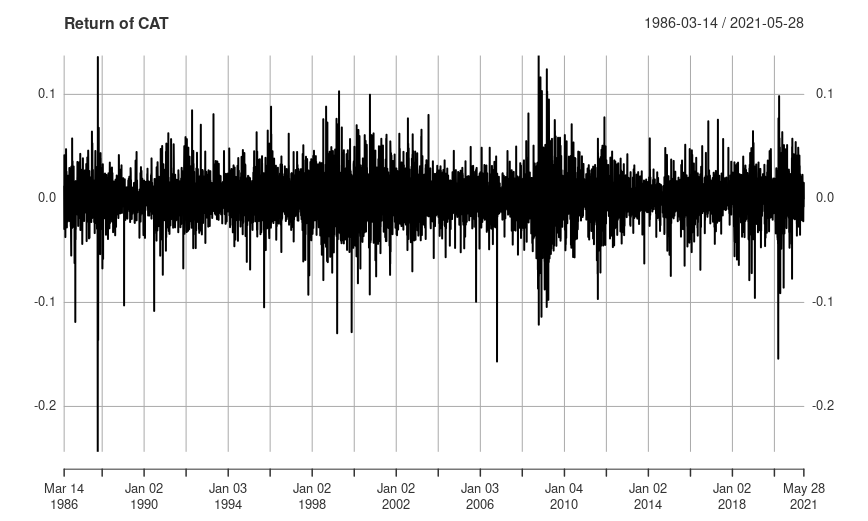
\includegraphics[width=\linewidth]{return_of_cat}
		\caption{Return of CAT as a function of time, at monthly intervals}
		\label{fig:returnCat}
	\end{subfigure}
	\caption{The returns of CAT over time.}
	\label{fig:return}
\end{figure}

\begin{figure}[h]
	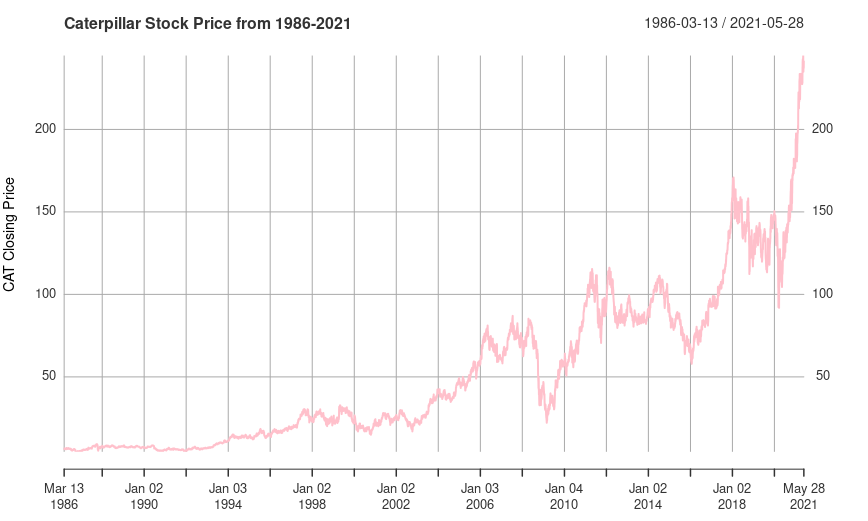
\includegraphics[width=\linewidth]{caterpillar_stock_price}
	\caption{The stock price of caterpillar as a function of time from 1986 - 2021}
	\label{fig:stockPrices}
\end{figure}



\end{document}
